% TBD by Wolfgang
\section{Style Viewers} 
\label{sec:viewers}
As we have shown earlier, the style views are the essence of the creative process so it's worth looking at this in its raw form. That's why we included some style viewer into the project to apply to this task. In this section we introduce them.

\subsection{Text Based viewer}
\label{sec:viewers.text}
As discussed earlier the styles are saved in a JSON file. Also these are made to intellectual by humans (???) we thought of a more pleasant way to view the style while developing. So we gave the style objects a print method. This method will print the style onto the current output of your python session, as can be seen in the figure below:

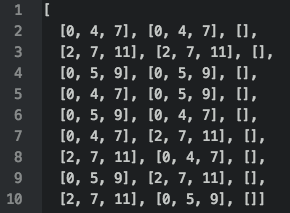
\includegraphics[scale=1]{Chapters/pic/text_print.png}

This figure shows the dummy style. The viewer orders all the style sequences according to their likelihood, starting with the most likely.  It also translates our numeric representation into a tonal representation for a given key (default key is C major).

That way one can easily see how the style will look like and if after applying the creative module an odd thing happened to the style, that would be harder to spot after the actual harmonizer. 

\subsection{MusicXML Creator}
\label{sec:viewers.musicxml}
Also faster and more visual would be to translate the style into a musicXML file and view it with your favorite musicXML viewer. We used MuseScore for that purpose. 

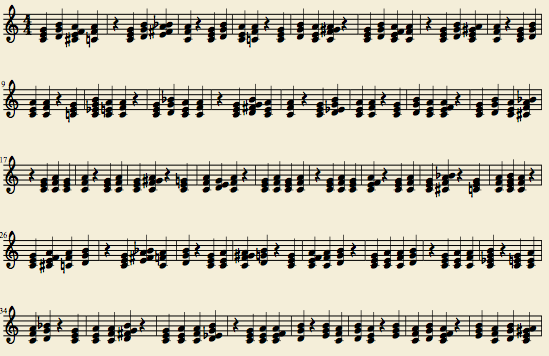
\includegraphics[scale=.5]{Chapters/pic/xml_print.png}

As seen in figure above we did it for the dummy style. To do that we used the $write_musicxml$ method of the visualizer. It does the same thing as the print method, that it orders the chord sequences starting with the most likely. But instead of printing it to the output it creates a musicxml file. For convenience we defined a bunch of default values, namely the key is C major, the duration of a tone is quarter pitch, as well as we use a four quarters rhythm. After every sequence we inserted a quarter break to indicate the end of a harmonization sequence.

With this visualization you have the major advantage that now you have standardized data structure and you are able to process them further. But mainly you want to view it in a score notation or listen to your creation.

This is where this ends, because now we have a wildly compatible format that can be used in to do any more complicated things you may want to do. 

\subsection{Extempore}
\label{sec:viewers.extempore}

TODO: Christoph (see also Section \ref{sec:tools.extempore})